\section{Theory of Real Time Systems}
The following section goes into the theories behind Real-Time Systems. Firstly brief explanations on some major technical terms used when speaking about real-time systems. \unsure{this is meta text to the chapter maybe? RTS shouldn't be a chapter}

A task that can be preempted is a task that can be interrupted, whereas a task that can't be preempted is a task that can't be interrupted.\todo{Lack of intro}

Each task has a corresponding period, the period is the interval within which the task should run, determined based on what is required for the task to fulfil its purpose, for the i-th task this is denoted $P_{i}$.


A task also has a corresponding deadline, Deadlines are the specific time before which a task should be completed, which will be determined based on what is required for the task to work optimally, this is denoted for the i-th task as $ D_{i} $. A deadline could be the same as the period of the task, however, if some task depends on the task, the deadline could be before the end of its period. 

Additionally, tasks have a worst-case execution time, which defines the maximum amount of time needed to complete its task, denoted as the i-th task $C_{i}$.

Tasks also have a worst-case response time, that defines the maximum time of time spent between it being released and when it has completed. This is different from the worst-case execution time, as this takes into account the amount of time spent while blocked by higher priority tasks. This can be calculated based on the tasks with higher priority. The following formula calculates the worst-case response time, in which hp is of a higher priority.

$R_{i} = C_{i} + \underset{j\in hp(i)}{\Sigma} \lceil\frac{R_{i}}{T_{j}}\rceil*C_{j} $

A system can be called schedulable if and only if all of its tasks can't exceed their respective deadlines. This can be calculated by assuming the worst-case execution time for all of the tasks and calculate the worst-case response time for all of the tasks. If the worst-case response time for all of the tasks doesn't exceed the deadline for all of the tasks, you can call that system schedule-able.

\todo{text about the different kinds of scheduling? needed. not needed. needed. not needed}
%\subsection{Cyclic executive scheduling}
%Perhaps the simplest form of scheduling, at least to understand, is Cyclic executive scheduling. Cyclic executive scheduling is a list of function calls in a never ending while loop. The list is contains all the necessary functions, arranged so that each task executes once in its period. The creation of the list is however a bit harder,   of functions needed to execute the program, this list 

%Event based scheduling

%Fixed priority scheduling 
%Earliest deadline first \unsure{what????}



%Technical terms that should be explained somewhere:

%Schedule-able meaning we can ensure that each task wont exceed their deadline. done

%Period meaning the interval in which a task is required to run once. done 

%Deadline a specific time before which a task should be completed. 

\subsection{\textbf{Fixed-Priority Scheduling}}\label{prioratySch}
The chosen platform supports two kinds of scheduling: Event-based scheduling and Fixed-Priority scheduling\cite{OILManual}.

Fixed Priority scheduling works by assigning a priority to each task. The scheduler will then chose to run the task with the highest priority first. However how we choose the priority of the different tasks,  that must be considered. If a task is given a priority based on their periods, and it's not schedulable then it is proven that it won't be schedulable on any other priority. Therefore the choice of priority is trivial, simply found according to the task's relative periods.

There are issues concerning this type of scheduling, namely priority inversion. Priority inversion exists if there is a task with higher priority waiting for lower priority tasks. This can occur if a low priority task holds a resource that the higher priority also needs, and it is unable to release until its finished some calculations. But the low priority task is then able to be preempted by other tasks with a relatively higher priority, however lower priority than the high priority task waiting for the release of a resource. This is illustrated in \ref{priorityInvertion}, where task 1 takes a resource, denoted by the purple line, which is also required by task 3. Since task 1 can't release the resource it is required that this task runs before task 3 can get its resource, however since task 1 is preempted by a higher priority, task 2, this makes task 3 wait on task 2, which is priority inversion.
\begin{figure}[H]
    \centering
    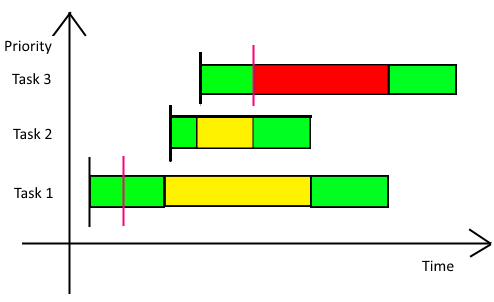
\includegraphics[width=0.7\textwidth]{Images/Analysis/priorityInvertion.png}
    \caption{Illustration of priority inversion}
    \label{priorityInvertion}
\end{figure}

This can be solved using priority inheritance. This is an inheritance of priority, if a task holds a resource, that a higher priority needs, it will be given the same priority as that task. 

We did not want to deal with event-based scheduling because we did not have a clear understanding of how we can ensure schedulability.\todo{this is the reason( selection by elimination), however, we cant write this, word it differently or find a better sounding reason}

\subsection{\textbf{OSEK Implementation Language}}\label{OILteo}
In this section, the report will go into detail with how the scheduling is supported. Most of the information about this can be found from this source\cite{OILManual}.

OIL stands for OSEK implementation language, it was made as an attempt to create an industry standard for an open-ended architecture for distributed control units in vehicles\cite{OILManual}. It is compiled with the code and provides some objects or constructions that aim to assist with the scheduling of the code. Since the OIL implementation is quite extensive, this rapport will limit its explanation to what is most relevant for this project. Since the project has decided to use Fixed-Priority Scheduling, see \ref{prioratySch}, the report will explain the important constructions in OIL files to support this form of scheduling, the report will, therefore, explain these three objects in the oil files.

\begin{itemize}
    \item{\textbf{Task}}
    The task in the OIL file is the primitive that the other objects control. The task within the OIL file is directly connected to a task within the c file, which describes the functionality of the task. The task within the OIL file describes the properties of the task. The interesting properties are: \textbf{The schedule value}, this value describes whether or not the task can be preempted, where FULL corresponds to a preemptable task and NON a non-preemptable task. \textbf{AUTO START} unsurprisingly this property determines whether or not the task auto starts. 
    \textbf{Priority} unsurprisingly this attribute describes the priority of a task, the lowest value corresponds to the lowest priority.
    %Random inforamtion:
    %Schedule value: The FULL value of this attribute corresponds to a preemptable task, the NON value to a nonpreemptable task.
    %AUTO START attribute: The AUTOSTART attribute determines whether the task is activated during the system startup procedure or not for some specific application modes. When set to TRUE, a list of application modes is defined in the APPMODE sub-attribute of type APPMODE\_TYPE. These define in which application modes the task is auto-started.
    %PRIORITY: This attribute is of type UINT32.  OSEK OS defines the lowest priority as zero (0); larger values of the PRIORITY attribute correspond to higher priorities.
    \item{\textbf{Counter}}
    A COUNTER is a global counter that should be incremented at a fixed interval and is necessary to be able to create an alarm. In the oil file, the ticks per call are declared as is its max value. In the NXT platform, a specific interrupt is used to implement the counter. \todo{maybe more verbose?}
    %Random inforamtion:
    %A COUNTER serves as a base for the ALARM mechanism
    %The counter in NXTOsek can be implemented with a hooking function called "user\_1ms\_isr\_type2" what interrupts every 1 ms, wherein one would count up the counter accordingly\cite{nxtOSEKAPI}.
    \item{\textbf{Alarm}}
    The alarm object controls the tasks, using a reference to a counter. It is the controlling object and its attributes dictate what happens when, so the following will be a brief overview of the alarms attributes. It has the attribute cycle time, which defines the period of a task. It also possesses an attribute called alarm time that defines the start delay before the alarm starts. And an attribute, ACTION, that defines what action should happen when the alarm expires\unsure{rings? calls? another word maybe}. Also, an AUTOSTART attribute that defines if the alarm should start itself and in what app modes it should do so.  An example of an alarm is given with some comments in \ref{code:AlarmExample}.
    
    \begin{lstlisting}[frame=single, label={code:AlarmExample}, caption={A example of an alarm in OIL}, xleftmargin=.00\textwidth, xrightmargin=.00\textwidth]
    ALARM AlarmExample
    {
        COUNTER = SysTimerCnt;
        /* reference to at counter */
        ACTION = ACTIVATETASK 
        /* the action attribute that decides what happens */
            {
                TASK = TaskExample;
                /* task(s) that the action is affecting */
            };
        AUTOSTART = TRUE
          /* autostart atribute, if false no further information is needed  */
        { 
            ALARMTIME = 250;
            /*delay before alarm starts the first time*/
            CYCLETIME = 400; 
            /* Task is executed every 400msec */
            APPMODE = appmode1;
            /* the appmode(s) wherein the alarm should autostart */
        };
    };
    \end{lstlisting}
   %Random information:
    %a Alarm has a reference to a counter
    %ACTION attribute: The ACTION attribute defines which type of notification is used when the alarm expires. This attribute is a parameterised ENUM can be used to ACTIVATETASK \{TASK\_TYPE TASK;\}
    %AUTOSTART: The AUTOSTART attribute of type BOOLEAN defines if an alarm is started automatically at system start-up depending on the application mode. 
    %OTHER:  ALARMTIME, i.e. the time when the ALARM shall expire first, the CYCLETIME, i.e. the cycle time of a cyclic ALARM 
\end{itemize}
%\subsubsection*{\textbf{task}}
%asd
%\subsubsection*{\textbf{Counter}}
%asd
%\subsubsection*{\textbf{Alerm}}
%asd

\subsection{\textbf{Time Constraints}}
There are 3 different kinds of time constraints on a system, soft, hard or firm time constraints. A hard real-time system is a system that is ruined by a missed deadline, e.g a system that gets destroyed if it misses a deadline. A firm real-taime system is a system that if a task misses its deadline, its calculations are unusable. A soft constrained real-time system is a system that can miss some of its deadlines and still produce useable calculations.


%We have concluded that our system is a soft Real-time system, i.e a system that can handle some missed deadlines without failing in its task. This conclusion is based on the task with the "hardest" deadline, the obstacle detection task

\subsection{\textbf{UPPAAL}}
We will be using the UPPAAL tool to model check our schedule to determine whether or not any of the projects tasks can exceed their deadlines.\todo{maybe we wont use uppaal??}

\subsection{\textbf{Communication primitives}}
Shared memory is going to be used as it is faster and simpler. It is more difficult to manage and understand the data locality. \todo{Huh?}

\subsection{\textbf{Shared Resources}} \info{prob not something that should be in to much detail}
 asd

%\subsection{Focus on real-time systems} \todo{This section has been moved and thus the section is not correct anymore. A bit of the section might be salvageable, but much of it will have to be removed or otherwise changed.}
%As written in section \ref{Requirements} the project involves a vehicle, that has to detect and react to the tasks ahead, like detecting bus stops or avoid obstacles, further described in the requirements. In general, the solution will be a control system for the vehicle which has to handle many different tasks. Therefore it is critical that the deadlines for the different functions are met if the actions that the control system takes is to be correct.

%For example, if the obstacle detection system were to miss a deadline, the vehicle could crash and thereby get destroyed, because it did not check if that it was driving into an obstacle.

%Since the control of the vehicle is to be autonomous and the environment can change, the vehicle has to react to the changes in real-time. The control system could, therefore, contain both hard and soft real-time deadlines, the difference is explained in\todo{add ref ref{theory of RTS}}. It is therefore important that a schedule is made to handle the many activities, and ensure that no computations are catastrophic for the control system. 

%It has been decided to focus on real-time systems. The decision of the control system will be hard- or soft real-time systems can be found in section \todo{add ref: ref{SoftwareDesign}}.